\section{Standard Architectures for Image Classification}
We are talking about networks for image classification. 
\subsection{GooglLeNet and Inception v1}
This is the network that won the competition in 2014 achieving a classification error of 6.7\%.
It is composed of the so called inception modules. The basic idea of the model is this:
\begin{center}
    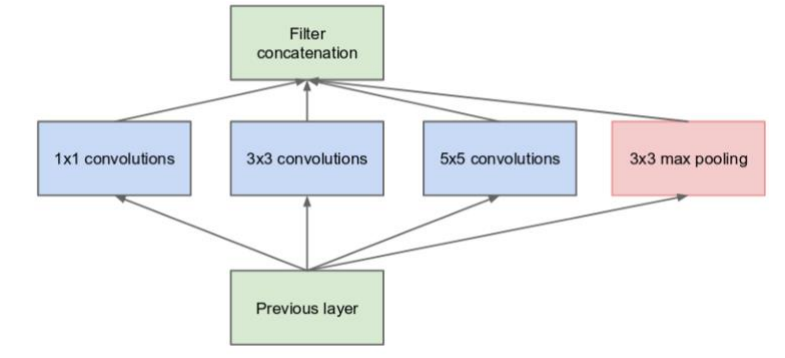
\includegraphics[width=0.7\textwidth]{images/googlenet.PNG}\par
\end{center}
A volume enters not a convolutional layer but in parallel multiple convolutional layers and a max pooling layer. Then all these outputs are combined together by concatenation to produce the layer output. There are multiple filter sizes in this way. The idea is that this was a sort of solution basing on the fact that it's hard to choose the filter size for feature extraction. 

Assuming you have a very small volume of 28x28x256, you perform some convolution (depending of the number of filters you will obviously have different numbers) with 128 filters 1x1, 192 3x3, 128 5x5 and 256 3x3 max pooling. To concatenate the output you perform some zero padding to preserve the spatial size, but the depth is increased. There are a large number of operations to be performed due to the large depth of the input of each convolutional layer (858 millions in this example). This is too expensive to compute, this network is expanding its depth preserving the spatial extent. To reduce the computational demand we can use the 1x1 convolution: we can stack 1x1 convolutional blocks right before 3x3 and 5x5 and after the max pooling. These 1x1 blocks are used as \textit{bottleneck layers}, in order to compress the number of features and create another non linearity. 
\begin{center}
    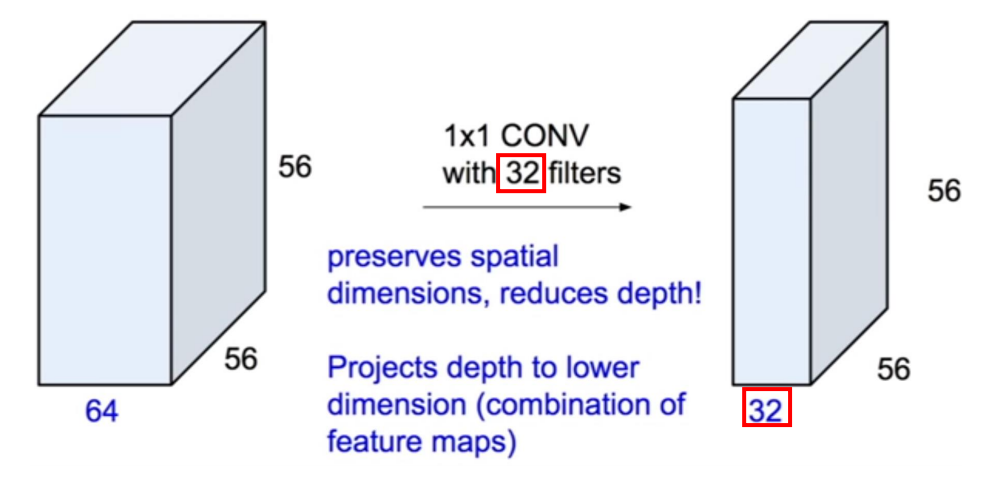
\includegraphics[width=0.6\textwidth]{images/1x1conb.PNG}\par
\end{center}
If you take 32 of these 1x1 filters, the output will have size 32 because each 1x1 filter will pass through the image providing one slice of the output. In this way the number of operations is significantly lower. There are overall 27 layers made of 9 inception modules; at the end you don't need a fully connected layer, there's only a global averaging pooling, a linear classifier and a softmax.
\begin{center}
    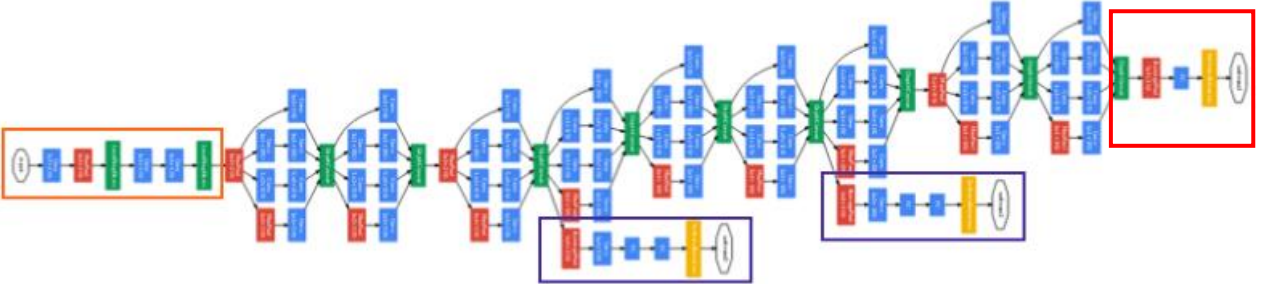
\includegraphics[width=0.7\textwidth]{images/incgoogle.PNG}\par
\end{center}
They introduced 2 extra classifiers. By introducing those classifiers, the loss to be minimized is no more the loss of the final network output but it's the sum of those losses and the final result is taken from that. This is just a trick for the vanishing gradient problem. 

\subsection{ResNet}
This model achieved 3\% performance the following year. There is a completely change of perspective in this network (which today has different versions). For the Inception the purpose was to handle feature patterns of multiple resolutions combining and replicating different sized filters; here the purpose was to design a network that was incredibly deep stacking more and more layers. They find out this:
\begin{center}
    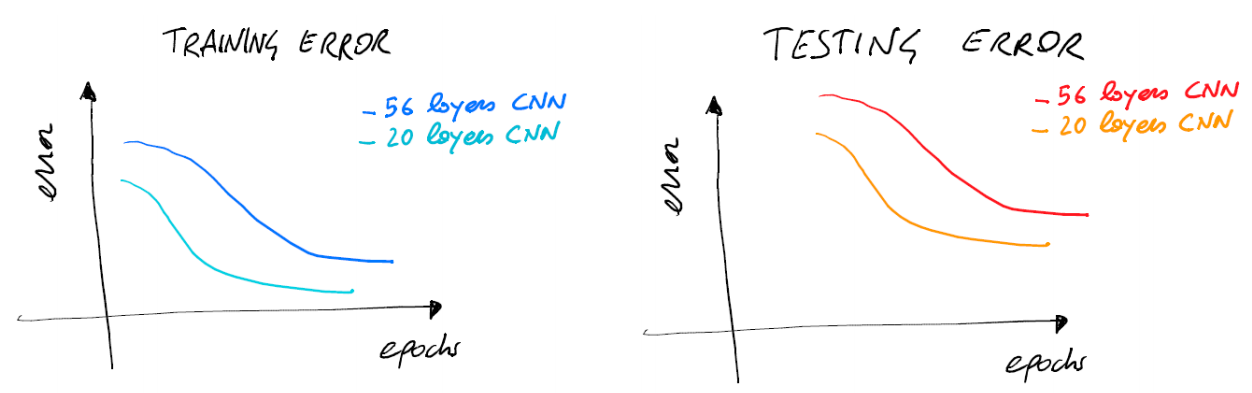
\includegraphics[width=0.9\textwidth]{images/resnet_error.PNG}\par
\end{center}
The testing error for a network with 20 layers and 56 layers had the same trend, but the one with 56 layers was larger. One can think that this is due to overfitting, but this is not the case because training and testing error should diverge but in this case this does not happen. Probably the reason is that you cannot explain the result as an overfitting problem, is just a problem of minimizing the loss function: training deeper networks is harder with respect to shallow networks. They added a skip connection, which corresponds to the identity, copying the parameters of the shallow network into the deeper network; if you are not good at learning deeper networks at least skip connections provide the identity. What happens is that you take the input of the two convolutional layers, which are the weights and non linearities, and what you do is summing the input to the output:
\begin{center}
    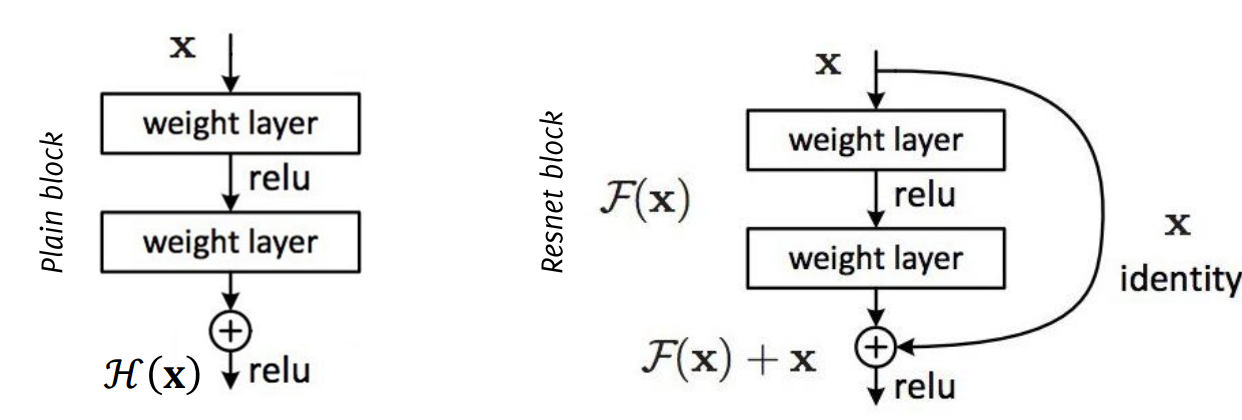
\includegraphics[width=0.6\textwidth]{images/resnet_skip.PNG}\par
\end{center}
This is something easier to train and the substantial increase in performance confirms that skip connections were a good idea. This is called \textbf{\textit{residual network}} because 
%if the ideal function that you would like to learn from a traditional architecture which is the same weights but without the skip connections,
if $H(x)$ is the function that you would like to learn than instead of learning $H(x)$ what you're learning is something like $\mathcal{F}(\mathbf{x})=\mathcal{H}(\mathbf{x})-\mathbf{x}$. Note that this does not add parameters to the network, it's just a copy and a sum, you are just letting the network solve a different learning problem. The weights in between the skip connections can be used to learn a "delta", a residual, $F(x)$ in order to improve the solution achieved by the shallow network.  There are a few consideration, in particular you have to be sure that the spatial extent is the same to perform the sum, so you have to do some padding to adjust the spatial extent. 

The substantial improvement achieved by the ResNet from the Inception (almost 50\% better in the classification error) probably can be justified that deeper networks are able to achieve lower errors, as expected. 

\subsection{DenseNet}
In this architecture there are skip connections everywhere. There are multiple blocks and inside each block the output is connected to each of the previous input for skip connections.

\subsection{Comparison}
You can see a model comparison using as variables the size of the parameters and the performance achieved. The AlexNet was the first actually and it was below 55\%, VGG had a lot of parameters and better performance but not incredibly good. 
\begin{center}
    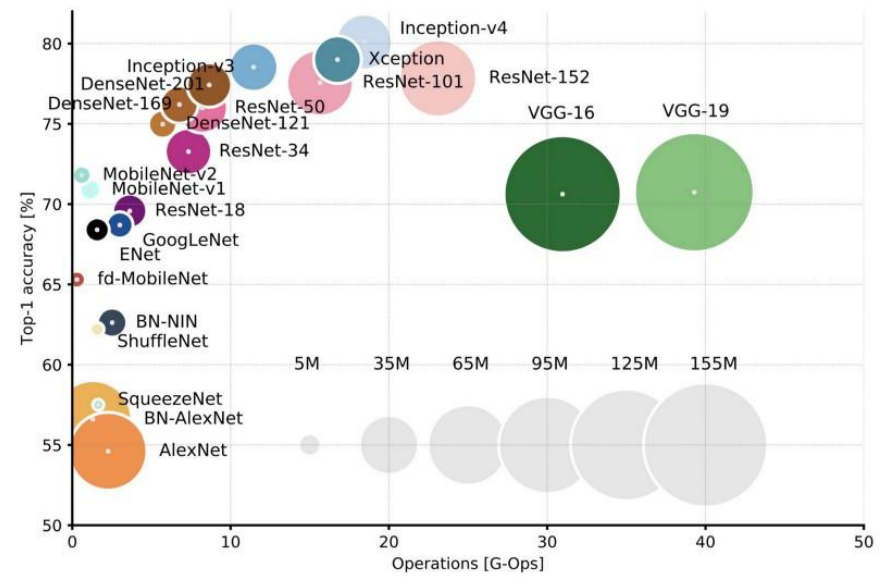
\includegraphics[width=0.75\textwidth]{images/model_comparison.PNG}\par
\end{center}
DenseNet and Inception are quite reduced but achieve very good performance. Inception models are the better performing, in particular the InceptionV4 that combines Inception and ResNet. Another important architecture is MobileNet which has very few parameters and it's very efficient but achieves decent performance; this uses separable convolutions and it's been designed for mobile purposes. 